\chapter{Implementation}

The extended Roofline method is implemented on a Haswell node which has one Intel (R) Xeon (R) processor E5 v3 @ 2.3GHz. The processor has 18 cores. The node has 32 GB of memory.
\section{Tools: PERF and LIBMSR}
The extended Roofline method is implemented as a library via the sampling method. For every sampling interval, the function $start\_collection()$ is called to collect all the necessary hardware events. This function is integrated with Perf and Libmsr.  

Perf is a powerful tool to measure the CPU activities via accessing the performance counters. The function $perf\_event\_open()$ is used to set up performance monitoring for core events. It generates a file descriptor corresponding to a hardware event that needs to be monitored \cite{24}. Six events namely instructions, CPU cycles, reference cycles, stall cycles for L2, stall cycles for LLC and stall cycles in total are measured during each sampling interval. The file descriptors of those events are grouped together which allows events to be monitored simultaneously.  

Perf is a good tool to measure the core events, however, it lacks of uncore supports. As a result, Libmsr \cite{25} is integrated into the library to measure the uncore events. Libmsr provides an interface that allows programmers to access the MSR directly. The uncore events include the read and write volumes of DRAM and LLC and the energy consumption of PKG and DRAM. 

\section{The Extended Roofline Method}

\begin{figure} [h] %hier können noch Positionierungswünsche angegeben werden
	\centering   % Alles weitere zentrieren
	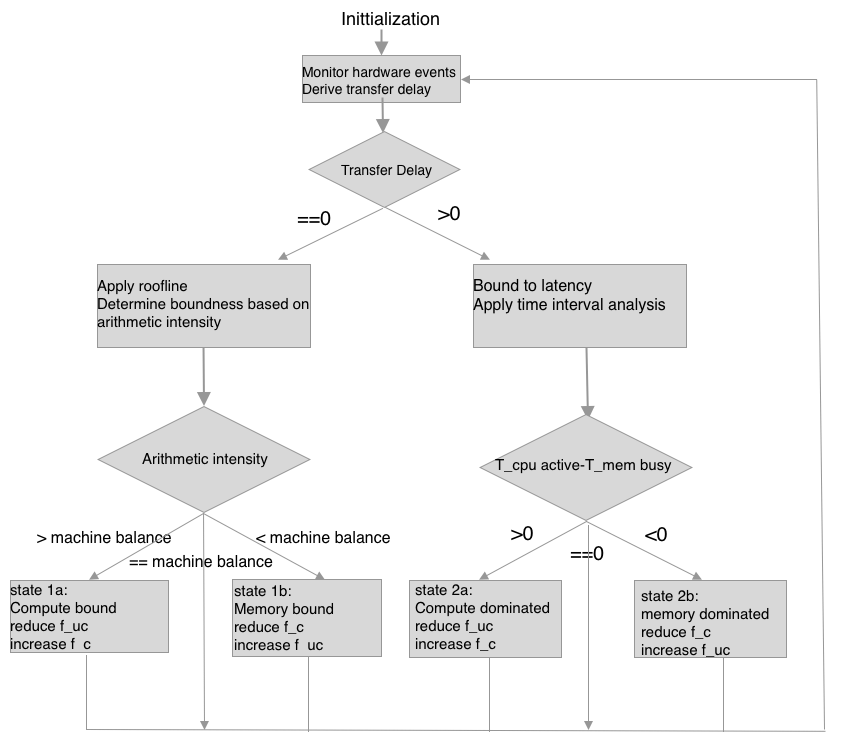
\includegraphics[width=12cm]{pictures/TIA}
	\caption{Combining the Roofline model with time interval analysis}
	%\label{fig3.7}  %Reihenfolge ist wichtig! Immer erst \caption{} dann \label{}
\end{figure}


Figure 4.1 shows the control logic of the extended Roofline method The first step is to initialise the core and uncore to their maximal frequency, $f_{c} $ = 2.8 GHz and $f_{uc} $ = 3.0 GHz. Then the hardware events are measured for each sampling interval. The sampling interval is set to 300 ms. 300 ms has minimum overhead comparing to other shorter intervals. Intervals longer than 300 ms may not detect the execution patterns correctly, e.g. it may not detect the change from memory-bound to compute-bound.
After collecting the hardware events, the function $calc\_roof()$ is called. This function first calculates the frequency of the core and uncore in Hertz, the CPU active and stall time in seconds, the busy and idle time of both DRAM and LLC in seconds and the PKG and DRAM power consumption in Watts. Then it executes the time interval analysis introduced in Section 3.3 and derives the transfer delay from the minimum of CPU stall time and memory idle time. 

If the transfer delay equals zero, the Roofline model is applied. Instead of using the FLOP/s to measure the kernel's performance in the Roofline model described in Chapter 3, the Instruction per second (IPS) is used. The reason is that not all applications perform floating-point operations only. The FLOP/s is not suitable for some applications that perform both integer operations and floating-point operations. As a result, the operational intensities of both LLC and DRAM are calculated by
\begin{equation}
operational\ intensity = \frac{instructions}{total\ data\ volume}
\end{equation}
The machine balance used in implementation is calculated as the ratio of the maximal instruction per second for the current time interval to the maximal memory bandwidth under the current uncore frequency. 
\begin{equation}
machine\ balance = \frac{maxIPS}{Full_{BW}}
\end{equation}
It is introduced in Chapter 3 that different applications have \textit{different} machine balances. The machine balance is calculated this way to guarantee it is the minimal intensity needed to reach the peak performance exclusively for the \textit{current} application in the time interval. By comparing the Equation (4.1) and (4.2), it ensures that no matter the application utilises FMA, SIMD and other ILP or not, the program always determines the correct performance bound. If the Equation (4.1) < Equation (4.2), the application is in state 1a which is compute-bound. If the Equation (4.1) > Equation (4.2), the application is in state 1b which is memory-bound. Otherwise, it is balanced.


When the transfer delay is greater than zero, the Roofline model is no longer suitable due to its inaccuracy. In this paper, this situation is defined as \textit{transfer delay bound}. The method continues to applying the time interval analysis to compare the CPU active time and memory busy time. If $T^{active}_{cpu}$ is greater than $T^{busy}_{mem}$, the system enters state 2a which is transfer delay bound dominated with computation. On the contrary, if $T^{active}_{cpu}$ is smaller than $T^{busy}_{mem}$, the system enters state 2b which is transfer delay bound dominated with memory.



\subsubsection{Side effects of frequency scaling on latency}

\begin{figure} [h] %hier können noch Positionierungswünsche angegeben werden
	\centering   % Alles weitere zentrieren
	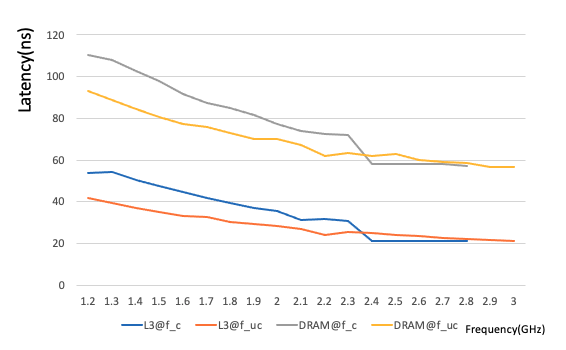
\includegraphics[width=15cm]{pictures/latency}
	\caption{L3 cache and DRAM latency change with respect to core/uncore frequency}
	%\label{fig3.9}  %Reihenfolge ist wichtig! Immer erst \caption{} dann \label{}
\end{figure}

As the clock frequencies are modified, the memory latency also changes. In the implementation, the transfer delay approximates to the latency. Figure 3.11 presents the change of the L3 cache and DRAM latency measured by the \textit{tinybench} \cite{38}. The core frequency is modified from 1.2 GHz to 2.8 GHz in steps of 0.1 GHz under the circumstance that the uncore frequency remains maximum. The uncore frequency are modified from 1.2 GHz to 3.0 GHz in steps of 0.1 GHz while keeping the core frequency at 2.8 GHz. The latency of DRAM and L3 cache decrease significantly with the increase of the core and uncore frequency. The latency of L3 decreases slower than DRAM with the increase of the core and uncore frequency. 

%The transfer delay is an essential part of the memory latency. Therefore, as the clock frequency increases, the transfer delay also increases.

\subsubsection{Modifying the CPU Clock Frequency}


%In this case, the uncore frequency is set to maximum and the core frequency is reduced by CORE\_STEP\_FREQ GHz, which is a global value that represents how much frequency will be changed in one tuning operation. Now I have to make sure that I did not over tune the core frequency. As I reduce the core frequency, the memory requests that the processor sends to the memory will be smaller. As a result, the memory idle time will be greater and we have a new time interval $T_{new}$ which is the time when memory is busy plus the new memory idle time. To determine whether the new time interval is too large that indicates an performance degradation, we simply compare $T_{new}$ with the execution time $T_{atMax}$ where the core frequency is maximum. If
%\begin{equation}
% T_{new} > T_{atMax} * (1 + ROOF\_THRESHOLD), 
%\end{equation}
%it shows that the new time interval exceeds the execution time when the core is maximum which indicates we have over reduced the core frequency. It heavily downgrades the performance, as a result the core frequency will be increased by CORE\_STEP\_FREQ. The ROOF\_THRESHOLD is a predefined threshold value.
%
The tuning of the CPU clock frequency contains two situations. One of them is the tuning does not concern any power cap. The other one is when there exists a power cap. The goal is to reduce the power consumption and in the meantime try not to downgrade the performance too much. 



\textbf{Without power cap}

For compute-bound state 1a, the $f_{uc}$ is reduced by \textit{UNCORE\_STEP\_FREQ} and the $f_c$ is set to maximum. For memory-bound state 1b, the $f_c$ is reduced by $CORE\_STEP\_FREQ$ and the $f_{uc}$ is set to maximum. For transfer delay bound with compute domination state 2a, the $f_{c}$ will be set to the maximum while the $f_{uc}$ is reduced by $UNCORE\_STEP\_FREQ$. As the uncore frequency decreases, the transfer delay increases respectively. Therefore, the time interval is increased. The new time interval is derived as $T_{new}$. A threshold needs to be defined to ensure the new time interval is not too large. Otherwise, it will cause performance downgrading. The threshold is set to $T_{atMax}* (1 + ROOF\_THRESHOLD)$. $T_{atMax}$ is the execution time where the uncore frequency is maximum. $ROOF\_THRESHOLD$ is a predefined value for precision tolerance. If
\begin{equation}
 T_{new} > T_{atMax} * (1 + ROOF\_THRESHOLD), 
\end{equation}
the core frequency will be re-added by $CORE\_STEP\_FREQ$.

For transfer delay bound with memory domination state 2b, the uncore frequency will be set to the maximum while the core frequency is reduced one step lower. The new time interval is calculated and compared with $T_{atMax}* (1 + ROOF\_THRESHOLD)$. The $T_{atMax}$ in this state is the execution time wherer the core frequency is maximum. If Equation 4.3 holds, it indicates that the new time interval exceeds the limit. Therefore, the core frequency is increased by $CORE\_STEP\_FREQ$.

\textbf{With power cap}

Under the circumstance that the power consumption has an upper limit, the tuning strategy should be reconsidered. For the state 2a, the $f_{uc}$ is decreased by $UNCORE\_STEP\_FREQ$ first. Since the uncore frequency is decreased, the system releases a small amount of power budget which can be used to increase the $f_c$. As the core and uncore frequency are modified simultaneously, the $T^{active}_{cpu}$, $T^{busy}_{mem}$, transfer delay, and the time interval also change. It is important to ensure the frequencies are not over-tuned. To do that, the algorithm compares $T^{active}_{cpu}$ with $T^{busy}_{mem}$ The CPU active time should be greater than the memory busy time. Otherwise, it suggests the application that is supposed to be compute dominated is changed to be memory dominated. If an over-tune is detected, the $f_{uc}$ is increased by $CORE\_STEP\_FREQ$. For state 2b, the tuning will be vice versa.
%Figure 3.10 shows the other case where it is compute bound. Since the processor dominates in the time interval, we have to divide it into two parts, one is the time that is bound to computation, and the other is bound to transfer delay. The transfer delay in this case is equal to the time when the processor stalls. The core frequency will be set to maximum while the uncore frequency is reduced one step lower. As I reduce the uncore frequency, the memory controllers that are responsible for data transfer between the memory and the processor will operate slower and make processor spend more time waiting for the data. Therefore the processor's stalling time will increase and we have to recalculate the time interval $T_{new}$ which is the time when processor is active plus the new processor's stalling time. Then I simply compare $T_{new}$ with the the execution time $T_{atMax}$ where the uncore frequency is maximum. If equation 3.3 holds, it shows that the new time interval exceeds the limit and I have to increase the uncore frequency one step higher.
%

